\documentclass{article}
\usepackage{tikz, comment}
\usepackage{pifont}
\usepackage{fontspec}
\usetikzlibrary{arrows, decorations.markings, decorations.pathreplacing}
\begin{comment}
:Title: Not defined yet
:Tags: pi;;moment;area using polar coordinates, polar integral formula ;cosine, cos ;polar form of a complex number
:Prob: 0.4251;0.421;0.4062;0.4032;0.394
:Slug: No name yet

Description Here.........
\end{comment}
\begin{document}\centering

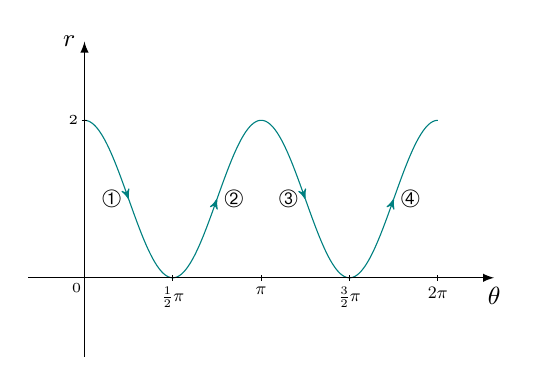
\begin{tikzpicture}[>=latex,xscale=.5/0.7, yscale=.5*2][font=\sf\small]

\draw[->, >=stealth', teal, samples=150, smooth, domain=0:pi/4, variable=\t]
plot ({\t}, {1+cos(2*\t r)}) -- ({pi/4}, {1+cos(2*(pi/4) r)});

\foreach \n in {1,3,5}
\draw[->, >=stealth', teal, samples=150, smooth, domain=(\n)*pi/4:(\n+2)*pi/4, variable=\t]
plot ({\t}, {1+cos(2*\t r)}) -- ({(\n+2)*pi/4}, {1+cos(2*((\n+2)*pi/4) r)});


\draw[teal, samples=150, smooth, domain=7*pi/4:2*pi, variable=\t]
plot ({\t}, {1+cos(2*\t r)});

%\draw[xstep=1cm,ystep=1cm,color=gray!80] (0, -1) grid (8, 8);
\foreach \x in {}
\draw (\x,2pt/6) -- (\x,-2pt/6)
node[anchor=north] {\tiny$\x$}
;
\draw ({1*pi/2},2pt/2) -- ({1*pi/2},-2pt/2)node[anchor=north, xshift=0, scale=0.7] {$\frac{1}{2}\pi$};
\draw ({pi},2pt/2) -- ({pi},-2pt/2)node[anchor= north, xshift=0, scale=0.7] {$\pi$};
\draw ({3*pi/2},2pt/2) -- ({3*pi/2},-2pt/2)node[anchor=north, xshift=0, scale=0.7] {$\frac{3}{2}\pi$};
\draw ({2*pi},2pt/2) -- ({2*pi},-2pt/2)node[anchor= north, xshift=0, scale=0.7] {$2\pi$};

\foreach \x in {}
\draw (\x,2pt*2) -- (\x,-2pt*2)
node[anchor=south] {\tiny$\x$}
;
\foreach \y in {2}
\draw (-2pt*0.7,\y) -- (2pt*0.7,\y)
node[anchor=east] {\tiny $\y$}
;

\draw[->] (-1, 0) -- ({2*pi+1}, 0)node[below] {\small $\theta$} ;
\draw[->] (0, -1) -- (0, 3)node[left] {\small $r$} ;

\node at ({1*pi/4 -0.3}, 1) {\ding{192}};
\node at ({1*pi/4+2*pi/4+0.3}, 1) {\ding{193}};
\node at ({1*pi/4+4*pi/4-0.3}, 1) {\ding{194}};
\node at ({1*pi/4+6*pi/4+0.3}, 1) {\ding{195}};

\node at (-0.2*0.7, -0.2/1.5) {\tiny$0$};

\end{tikzpicture}\hskip0.5cm
\end{document}